% Experiments and Results (owner M). Sources:
%   experiments/results/systems_s1_s2_s3.json  (every S2/S3 cell, CIs, floors)
%   experiments/asvspoof_retention_summary.json (S1 English)
%   results/s1_norm/stage1__*.json         (S1 on the normalised code-mixed sets)
%   experiments/results/lowlevel_cue_check_*.json (shortcut floors)

\section{Experiments and Results}
\label{sec:results}

\subsection{The generalisation gap}
\label{sec:gap}

S1 is a strong English detector. On the ASVspoof 2019 LA evaluation set it reaches
0.85\% EER (AUC 0.994) over attacks it never saw in training; an independent
re-scoring of the same checkpoint on the same 71{,}237 clips gives 0.90\%
[0.83, 0.99]. On the same
code-mixed sets that S2 and S3 are measured on, it fails every one
(Table~\ref{tab:gap}): 41.67--48.21\% EER on clean audio and 44.15--58.42\% over the
telephone channel, against shortcut floors of 5.17--31.21\% and 10.01--25.79\%. No
cell comes close to its floor.

\begin{table}[t]
\centering
\caption{S1, trained on English only, on the normalised code-mixed sets. Floors are
the shortcut floors of Table~\ref{tab:floors}.}
\label{tab:gap}
\small
\begin{tabular}{@{}llrrr@{}}
\toprule
Test set & Condition & EER (\%) & AUC & Floor \
\midrule
ASVspoof LA eval (English) & clean   & 0.85  & 0.994 & -- \
\midrule
Eval pool (XTTS)           & clean   & 48.21 & 0.557 & 5.17 \
CM04 (Tortoise)            & clean   & 41.67 & 0.597 & 31.21 \
RVC test                   & clean   & 43.46 & 0.546 & 28.76 \
Eval pool (XTTS)           & channel & 58.42 & 0.381 & 10.01 \
CM04 (Tortoise)            & channel & 44.15 & 0.561 & 25.79 \
RVC test                   & channel & 55.57 & 0.425 & 22.46 \
\bottomrule
\end{tabular}
% results/s1_norm/stage1__*.json
\end{table}

The AUCs show how it fails. S1 does not mainly miss the fakes; it rejects the real
speakers. It calls 94.8\% of genuine Hindi--English speech fake on clean audio, with
a median $P(\text{genuine})$ of 0.0005. The same model at the same operating point
rejects 0.37\% of genuine English, so changing the language and the recording domain
raises its false-alarm rate on real speech by a factor of 256.
Over the telephone channel every AUC falls
below 0.5, so the clones look \emph{more} genuine to S1 than the real speakers do.
In a deployment this is the more damaging error: nearly every genuine caller would
be flagged. The model's notion of genuine speech is tied to the recording conditions
and language of its training data rather than to properties of synthesis. Because
ASVspoof is studio read speech and MUCS is lecture audio, this gap combines language
shift with recording-domain shift, and we do not claim it isolates code-mixing.

\subsection{Shortcut floors}
\label{sec:floors}

Before reading any code-mixed result we measured how far cheap statistics get on
each test set (Table~\ref{tab:floors}). On the corpus as first built, before level
normalisation, the eight statistics reached 1.39\% EER on the evaluation pool. A
headline number of 1.34\% from our first clean adapter therefore had no margin over
a logistic regression, and we withdrew it. Normalising to $-23$~dBFS raises the
floor to 5.17\%. The remaining separation comes from zero-crossing rate and RMS
variability, a trace of lecture recording set against vocoder output that
normalisation cannot remove. Every code-mixed result below is reported against the
floor of its own set and condition.

\begin{table}[t]
\centering
\caption{Shortcut floors: EER (\%) of a logistic regression on eight signal
statistics. A detector must beat the floor of its set to count as evidence.}
\label{tab:floors}
\small
\begin{tabular}{@{}lrr@{}}
\toprule
Test set & Clean & Channel \\
\midrule
Eval pool (XTTS, seen tool)        & 5.17  & 10.01 \\
CM04 (Tortoise, unseen tool)       & 31.21 & 25.79 \\
RVC test (unseen speakers)         & 28.76 & 22.46 \\
\bottomrule
\end{tabular}
\end{table}

\begin{figure}[t]
\centering
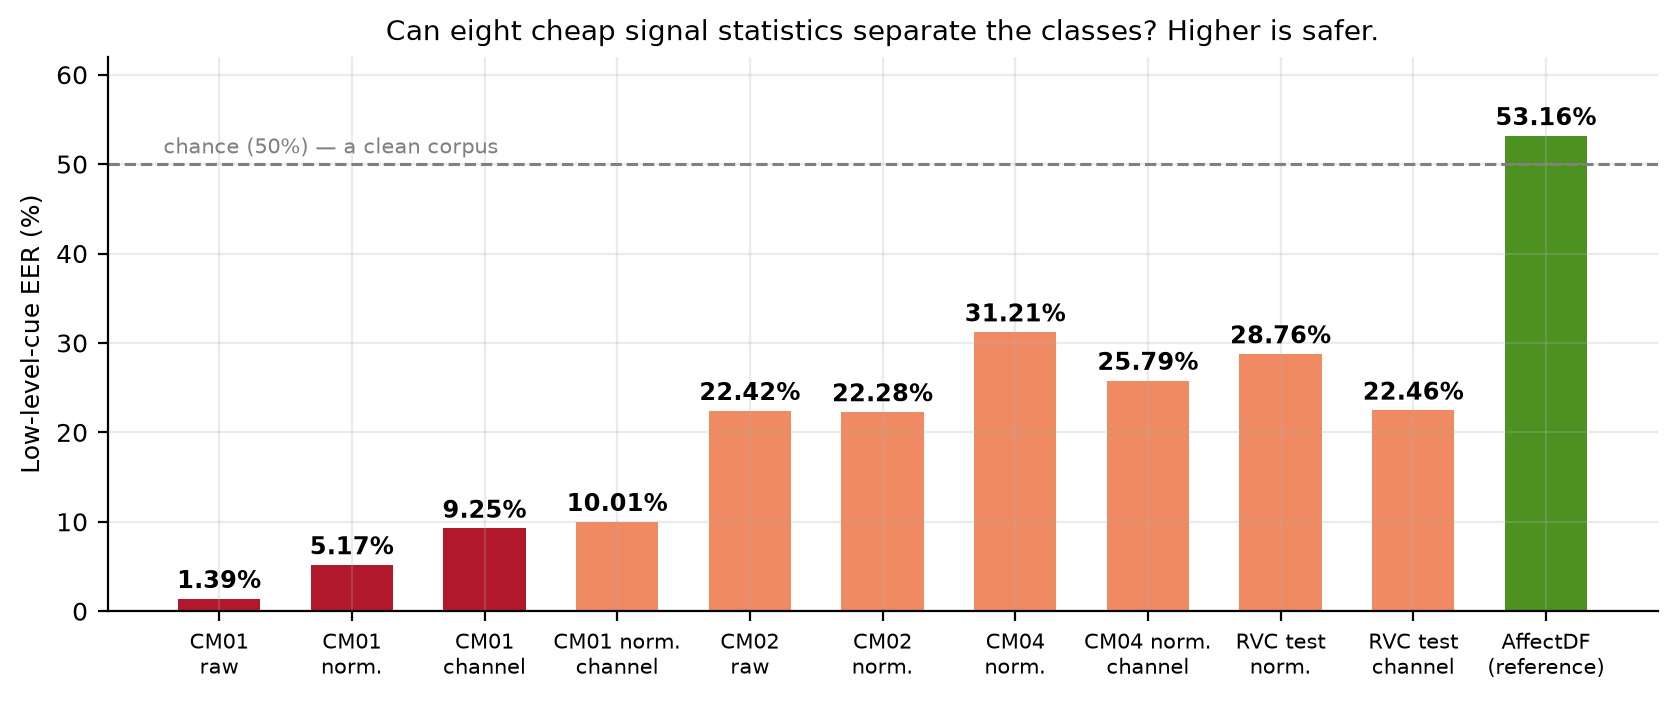
\includegraphics[width=\columnwidth]{figures/shortcut_gate.png}
\caption{Shortcut gate: EER of the eight-statistic logistic regression against
chance, per set and condition.}
\label{fig:gate}
\end{figure}

\subsection{Adaptation and native training}
\label{sec:main}

Table~\ref{tab:main} gives every S2 and S3 model on every test set, in its own
training condition, and Fig.~\ref{fig:systems} shows the same numbers against the
floors.

\begin{table*}[t]
\centering
\caption{EER (\%) with 95\% bootstrap confidence intervals. \textbf{Bold}: the interval's
upper bound is below the shortcut floor of that set and condition. \textit{Italic}:
it is not, so the cell is not evidence of learning. English has no floor.}
\label{tab:main}
\small
\begin{tabular}{@{}lllcccc@{}}
\toprule
System & Training attacks & Condition & Eval pool (XTTS) & CM04 (Tortoise) & RVC test & English \\
\midrule
\multicolumn{3}{@{}l}{\emph{Shortcut floor, clean}}   & 5.17  & 31.21 & 28.76 & -- \\
\multicolumn{3}{@{}l}{\emph{Shortcut floor, channel}} & 10.01 & 25.79 & 22.46 & -- \\
\midrule
S2 LoRA   & XTTS       & clean   & \textbf{1.46} {\scriptsize[1.01, 1.94]} & \textbf{5.44} {\scriptsize[4.05, 6.57]}   & \textbf{23.91} {\scriptsize[20.33, 27.64]} & 15.83 {\scriptsize[15.54, 16.04]} \\
S2 LoRA   & XTTS       & channel & \textbf{4.41} {\scriptsize[3.78, 5.19]} & \textit{28.16} {\scriptsize[25.44, 30.20]} & \textit{29.56} {\scriptsize[26.49, 32.79]} & 2.55 {\scriptsize[2.43, 2.67]} \\
S2 LoRA   & XTTS + RVC & clean   & \textbf{1.99} {\scriptsize[1.47, 2.45]} & \textbf{12.01} {\scriptsize[10.42, 13.64]} & \textbf{5.01} {\scriptsize[3.55, 6.95]}   & 3.75 {\scriptsize[3.63, 3.91]} \\
S2 LoRA   & XTTS + RVC & channel & \textbf{2.75} {\scriptsize[2.22, 3.37]} & \textit{30.99} {\scriptsize[28.72, 33.84]} & \textbf{5.01} {\scriptsize[3.39, 6.95]}   & 2.42 {\scriptsize[2.31, 2.54]} \\
\midrule
S3 native & XTTS       & clean   & \textbf{1.46} {\scriptsize[1.08, 1.82]} & \textbf{27.72} {\scriptsize[25.77, 30.14]} & \textit{45.07} {\scriptsize[40.87, 50.24]} & 56.42 {\scriptsize[55.81, 56.93]} \\
S3 native & XTTS       & channel & \textbf{1.92} {\scriptsize[1.43, 2.40]} & \textbf{13.71} {\scriptsize[12.30, 15.23]} & \textit{32.15} {\scriptsize[28.43, 35.55]} & 55.83 {\scriptsize[55.31, 56.41]} \\
S3 native & XTTS + RVC & clean   & \textbf{0.83} {\scriptsize[0.53, 1.14]} & \textbf{21.39} {\scriptsize[18.39, 24.58]} & \textbf{8.24} {\scriptsize[5.66, 10.51]}  & 50.90 {\scriptsize[50.45, 51.35]} \\
S3 native & XTTS + RVC & channel & \textbf{1.79} {\scriptsize[1.44, 2.26]} & \textit{31.67} {\scriptsize[28.20, 34.57]} & \textbf{5.98} {\scriptsize[4.19, 8.09]}   & 52.25 {\scriptsize[51.58, 52.86]} \\
\midrule
S1        & ASVspoof   & --      & \multicolumn{3}{c}{see Table~\ref{tab:gap}} & 0.85 \\
\bottomrule
\end{tabular}
\end{table*}

\begin{figure*}[t]
\centering
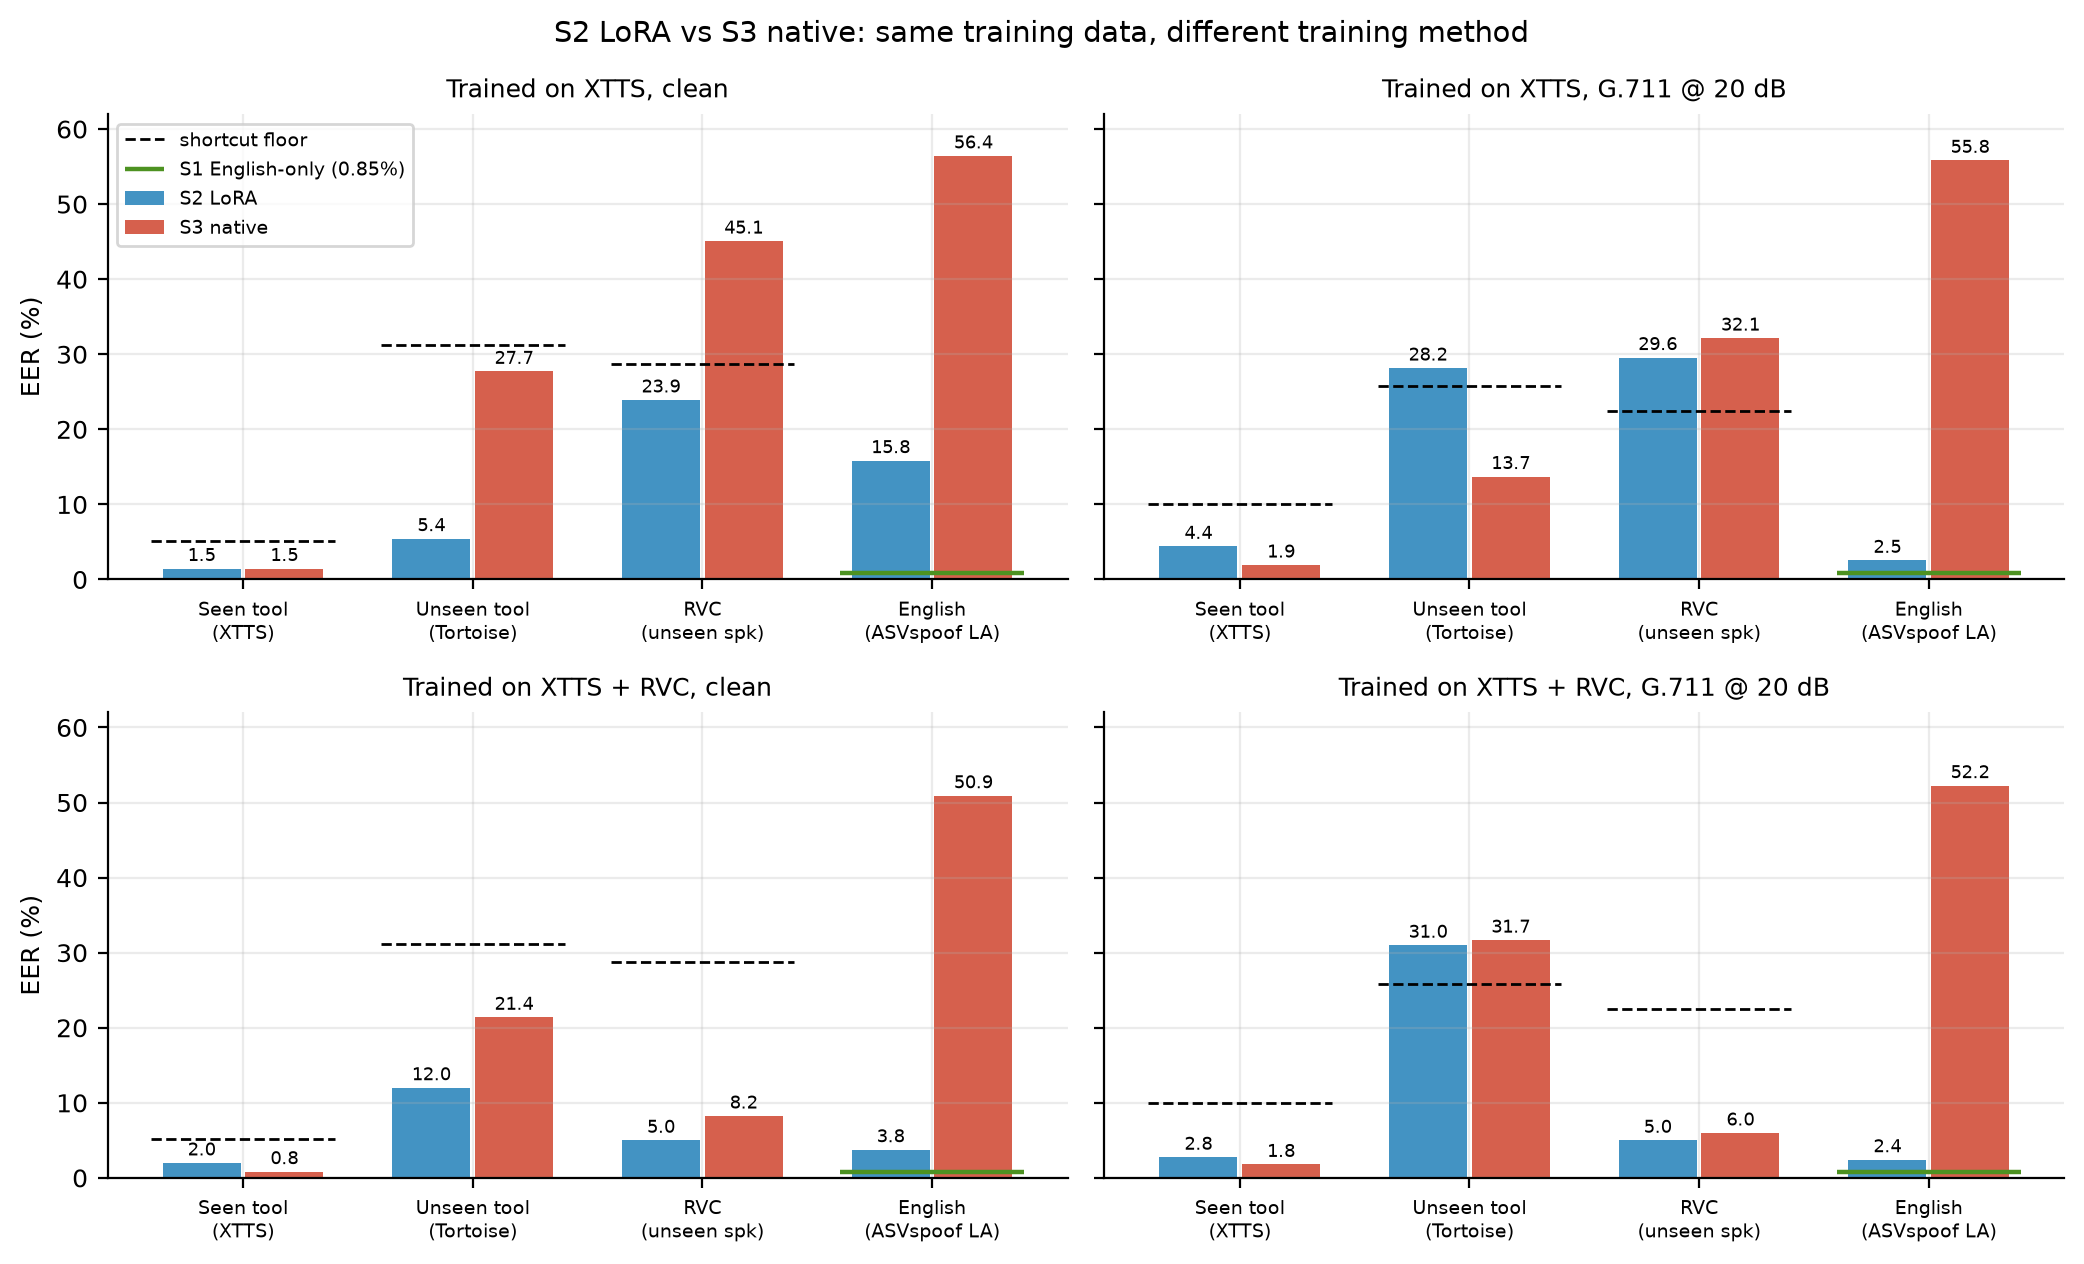
\includegraphics[width=\textwidth]{figures/systems_s2_s3.png}
\caption{S2 (LoRA) and S3 (native) trained on the same data, per training variant.
Dashed lines are shortcut floors; the green line is S1 on English.}
\label{fig:systems}
\end{figure*}

Five findings follow.

\textbf{1. A 1\% adapter closes the gap on the seen tool.} Every S2 model beats its
evaluation-pool floor, at 1.46--1.99\% clean and 2.75--4.41\% over the telephone
channel.
Moving 1.13\% of the weights takes the detector from chance to below the floor on
unseen speakers.

\textbf{2. The adapter must be trained on the deployment channel.} Before
normalisation, an adapter trained on clean audio and scored on channel-rendered
audio rose from 1.34\% to 38.58\% EER, passing most clones as genuine; its cue lay
above 4~kHz, which a narrowband codec removes. Training on channel-rendered audio
recovered 3.89\%. After normalisation, both channel-matched S2 models clear the
10.01\% channel floor. We therefore train and score each model in the condition it
will be used in.
% pre-normalisation figures: docs/results/channel_matched_v1.md

\textbf{3. Attack diversity is not free.} Adding RVC conversions to S2's training
data cuts RVC EER from 23.91\% to 5.01\% clean and from 29.56\% to 5.01\% over the
channel, on speakers unseen as source or target. It also raises EER on the unseen
Tortoise attack, from 5.44\% to 12.01\% clean and from 28.16\% to 30.99\% over the
channel (Fig.~\ref{fig:ablation}). Covering one attack family moved the decision
boundary away from another.

\begin{figure}[t]
\centering
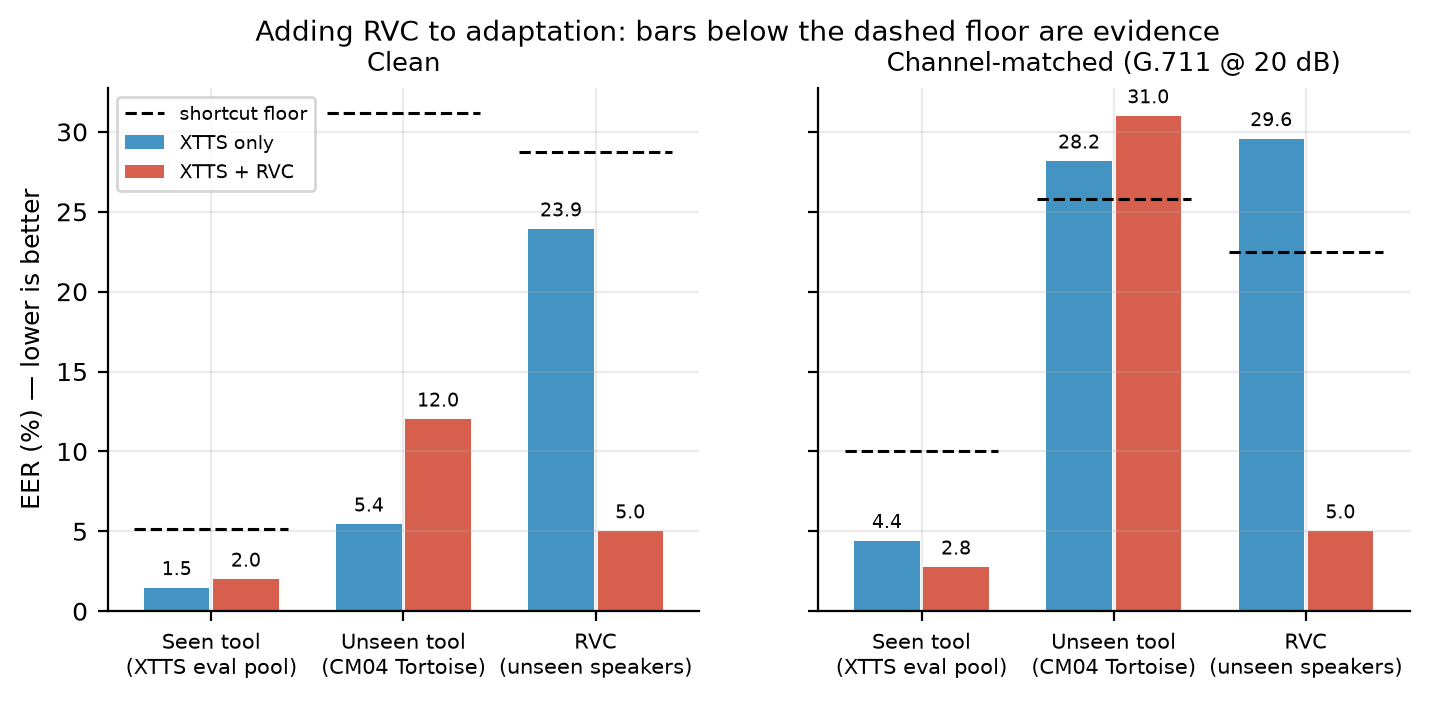
\includegraphics[width=\columnwidth]{figures/ablation_rvc.png}
\caption{Adding RVC to S2's adaptation data, clean and channel-matched. Bars below
the dashed floor are evidence.}
\label{fig:ablation}
\end{figure}

\textbf{4. Native training wins on its own data and loses English.} S3 is the most
accurate model on the seen tool, reaching 0.83\% clean with XTTS and RVC in training
against 1.99\% for the matching S2. On English it sits at 50.90--56.42\% EER, which
is chance, in every variant. S2 keeps English at 2.42--3.75\% in three of four
variants; the clean XTTS-only adapter is the exception at 15.83\%. The collapse is
the English-to-code-mixed gap of Sec.~\ref{sec:gap} run in reverse: each model
learns its own training domain's notion of genuine speech. Adaptation keeps S1's
notion and extends it, which is why S2, not S3, is the system we deploy.

\textbf{5. The unseen tool over a telephone line is not solved.} On clean audio,
all four models beat the Tortoise floor, S2 XTTS-only best at 5.44\%. Over the
channel only one of four does, S3 XTTS-only at 13.71\%; the deployed model, S2 with XTTS and
RVC in channel-matched training, scores 30.99\% against a 25.79\% floor. Detecting a
synthesis tool never seen in training, after the telephone channel has removed high
frequencies, remains open, and we report it as the main limitation of this work.

\subsection{What the detector responds to}
\label{sec:probe}

The detector reads a raw waveform and has no hand-written features, so we probe it
by changing one property of the audio at a time and reading the score. All numbers
here are the deployed S2 model on the five held-out demo calls, scored exactly as
the live system scores a call.

\textbf{Not language, words or prosody.} Cutting a code-mixed call into 100~ms
pieces and shuffling them destroys word order, grammar, code-mixing and sentence
melody. In the deployment condition the verdicts do not move: the genuine call
stays at $P(\text{genuine}) = 0.999$ and the XTTS clone at 0.000. The same point
holds inside one language, where shuffling is not involved at all: an RVC
conversion keeps its source speaker's exact words, timing and code-mixing, and the
pair scores 1.000 against 0.002. On clean studio English the shuffle probe is not
informative, because both S1 and this model read the discontinuities it introduces
as artefacts and reject the genuine clip; both survive a 500~ms shuffle.

\textbf{The cue is short and lives in the phase.} Evidence survives 100~ms
shuffling, weakens at 25~ms and is gone at 5~ms, which is shorter than one
vocal-cord cycle. Scrambling the phase while keeping the magnitude spectrogram
exactly drops genuine audio from 0.999 to 0.000, whereas an analyse-and-resynthesise
round trip that preserves phase changes nothing. Level changes, an extra telephone
codec pass and noise down to 10~dB SNR also leave the verdicts intact.

\textbf{The decision forms early in the encoder.} Separating genuine from cloned
windows along the class-mean direction, scored on held-out windows, gives AUC 0.901
at the convolutional output, which sees 25~ms and no context, and saturates by
transformer layer 3. In wav2vec~2.0 linguistic content emerges in the middle and
upper layers, so the decision is essentially complete before it exists.

\textbf{Language is not the cue.} Real English from ASVspoof, through this
Hinglish-adapted model, scores a mean of 1.000 and is called real in 100\% of
clips, while English attacks are caught in 84.8\%.

Together these say the model reads how the waveform was produced, at the scale of a
single vocal-cord pulse, rather than what is being said or in which language.
% src/inference/interpretability.py; experiments/results/interpretability.json
% docs/results/interpretability_v1.md

\subsection{Summary}
The best all-round system is S2 trained on XTTS and RVC in the channel condition. It
beats its floor on the seen tool (2.75\%) and on RVC (5.01\%), keeps English at 2.42\%,
and fails only on the unseen tool over the channel. It is the model used in the live
call system of Sec.~\ref{sec:system}.
